\documentclass[11pt,a4paper,oneside]{book}
\usepackage{a4wide}                     % Iets meer tekst op een bladzijde
\usepackage[dutch]{babel}               % Voor nederlandstalige hyphenatie (woordsplitsing)
\usepackage{amsmath}                    % Uitgebreide wiskundige mogelijkheden
\usepackage{amssymb}                    % Voor speciale symbolen zoals de verzameling Z, R...
\usepackage{makeidx}                    % Om een index te maken
\usepackage{url}                        % Om url's te verwerken
\usepackage{graphicx}                   % Om figuren te kunnen verwerken
\usepackage[small,bf,hang]{caption}     % Om de captions wat te verbeteren
\usepackage{xspace}                     % Magische spaties na een commando
\usepackage[latin1]{inputenc}           % Om niet ascii karakters rechtstreeks te kunnen typen
\usepackage{float}                      % Om nieuwe float environments aan te maken. Ook optie H!
\usepackage{flafter}                    % Opdat floats niet zouden voorsteken
\usepackage{listings}                   % Voor het weergeven van letterlijke text en codelistings
\usepackage[round]{natbib}              % Voor auteur-jaar citaties.
\usepackage[nottoc]{tocbibind}		% Bibliografie en inhoudsopgave in ToC; zie tocbibind.dvi
\usepackage{eurosym}                    % om het euro symbool te krijgen
\usepackage{textcomp}                   % Voor onder andere graden celsius
\usepackage{fancyhdr}                   % Voor fancy headers en footers
\usepackage[Gray,squaren,thinqspace,thinspace]{SIunits} % Om elegant eenheden te zetten
\usepackage[version=3]{mhchem}          % Voor elegante scheikundige formules

% Volgend package is niet echt nodig. Het laat echter toe om gemakkelijk elektronisch
% te navigeren in je pdf-document. Deze package moet altijd als laatste ingeladen worden.
\usepackage[a4paper,plainpages=false]{hyperref}    % Om hyperlinks te hebben in het pdfdocument.


%%%%%%%%%%%%%%%%%%%%%%%%%%%%%%
% Algemene instellingen van het document.
%%%%%%%%%%%%%%%%%%%%%%%%%%%%%%

% De splitsingsuitzonderingen
\hyphenation{back-slash split-sings-uit-zon-de-ring}

%\bibpunct{(}{)}{;}{y}{,}{,}             % Auteur-jaar citaties -- zie natbib.dvi voor meer uitleg; niet echt nodig

% Het bibliografisch opmaak bestand.
% ZORG ERVOOR DAT bibliodutch.bst ZICH IN JE WERKDIRECTORY BEVINDT!!!
\bibliographystyle{bibliodutch}

\setlength{\parindent}{0cm}             % Inspringen van eerste lijn van paragrafen is niet gewenst.

\renewcommand{\baselinestretch}{1.2} 	% De interlinie afstand wat vergroten.

\graphicspath{{figuren/}}               % De plaars waar latex zijn figuren gaat halen.

\makeindex                              % Om een index te genereren.

\setcounter{MaxMatrixCols}{20}          % Max 20 kolommen in een matrix

% De headers die verschijnen bovenaan de bladzijden, herdefinieren:
\pagestyle{fancy}                       % Om aan te geven welke bladzijde stijl we gebruiken.
\fancyhf{}                              % Resetten van al de fancy settings.
\renewcommand{\headrulewidth}{0pt}      % Geen lijn onder de header. Zet dit op 0.4pt voor een mooie lijn.
\fancyhf[HL]{\nouppercase{\textit{\leftmark}}} % Links in de header zetten we de leftmark,
\fancyhead[HR]{\thepage}                % Rechts in de header het paginanummer.
% Activeer de volgende lijn en desactiveer de vorige om paginanummers onderaan gecentreerd te krijgen.
%\fancyhf[FC]{\thepage}                  % Paginanummers onderaan gecentreerd.

% PDF specifieke opties, niet strict noodzakelijk voor een thesis.
% Is hetgeen verschijnt wanneer je in acroread de documentproperties bekijkt.
\hypersetup{
    pdfauthor = {Gaspard Lequeux},
    pdftitle = {Een Introductie tot het Zetsysteem LaTeX},
    pdfsubject = {Cursus LaTeX opgebouwd als typevoorbeeld voor het schrijven van een thesis.},
    pdfkeywords = {LaTeX, zetsysteem, thesis, eindwerk}
}


% Het volgende commando zou ervoor moeten zorgen dat er een witte ruimte wordt gelaten tussen
% elke paragraaf. Het zorgt ervoor dat er echter teveel witte ruimte komt boven en onder de
% verschillende titels, gemaakt met \section, subsection...
%%\setlength{\parskip}{0ex plus 0.3ex minus 0.3ex}

% Vandaar dat we expliciet aangeven wanneer we wensen dat een nieuwe paragraaf begint:
% \par zorgt ervoor dat er een nieuwe paragraaf begint en
% \vspace zorgt voor vertikale ruimte.
\newcommand{\npar}{\par \vspace{2.3ex plus 0.3ex minus 0.3ex}}

%%%%%%%%%%%%%%%%%%%%%%%%%%%%%%
% Nieuwe commando's
%%%%%%%%%%%%%%%%%%%%%%%%%%%%%%

% De differentiaal operator
\newcommand{\diff}{\ensuremath{\mathrm{d}}} 

% Super en subscript
\newcommand{\supsc}[1]{\ensuremath{^{\text{#1}}}}   % Superscript in tekst
\newcommand{\subsc}[1]{\ensuremath{_{\text{#1}}}}   % Subscript in tekst

% Chemische formule font:
\newcommand{\ch}[1]{\ensuremath{\mathrm{#1}}\xspace}	 
% Chemische pijl naar rechts:
\newcommand{\chpijlr}{\ensuremath{\hspace{1em}\longrightarrow\hspace{1em}}}
% Chemische pijl naar links:
\newcommand{\chpijll}{\ensuremath{\hspace{1em}\longleftarrow\hspace{1em}}}
% Chemische pijl naar links en rechts:
\newcommand{\chpijllr}{\ensuremath{\hspace{1em}\longleftrightarrow\hspace{1em}}}

\newcommand{\vt}[1]{\ensuremath{\boldsymbol{#1}}} % vector in juiste lettertype
\newcommand{\mx}[1]{\ensuremath{\mathsf{#1}}}	  % matrix in juiste lettertype

% Het latex logo in een eenvoudiger commando steken
\newcommand{\latex}{\LaTeX\xspace}

% Het BibTeX logo
\newcommand{\bibtex}{\textsc{Bib}\TeX\xspace}

% Niew commando om bestandnamen anders weer te geven
\newcommand{\bestand}[1]{\lstinline[basicstyle=\sl]{#1}\xspace}

% Niew commando om commando tekst weer te geven
\newcommand{\command}[1]{\lstinline[basicstyle=\tt]{#1}\xspace}
\newcommand{\commandx}[1]{\index{#1}\lstinline[basicstyle=\tt]{#1}\xspace}

%\lstset{morecomment={\%}}
% Commando om latex commando`s weer te geven (x: voor indexing)
%\newcommand{\lcommand}[1]{\lstinline[basicstyle={\tt},{language=[LaTeX]TeX}]{#1}\xspace}
\newcommand{\lcommand}[1]{\lstinline[basicstyle={\tt}]{#1}\xspace}
\newcommand{\lcommandx}[1]{\index{#1}\lstinline[basicstyle=\tt]{#1}\xspace}


% Niew commando om vreemde taal weer te geven (hint: dit commando kan gebruikt
%   worden om latijnse namen, die ook cursief moeten staan, weer te geven.
\newcommand{\engels}[1]{\textit{#1}\xspace}
\newcommand{\engelsx}[1]{\index{#1}\textit{#1}\xspace}

% Niew commando om iets te benadrukken en tegelijkertijd in de index te steken.
\newcommand{\begrip}[1]{\index{#1}\textbf{#1}\xspace}

% Nieuw commando om figuren in te voegen. Gebruik:
% \mijnfiguur[H]{width=5cm}{bestandsnaam}{Het bijschrift bij deze figuur}
\newcommand{\mijnfiguur}[4][ht]{            % Het eerste argument is standaar `ht'.
    \begin{figure}[#1]                      % Beginnen van de figure omgeving
        \begin{center}                      % Beginnen van de center omgeving
            \includegraphics[#2]{#3}        % Het eigenlijk invoegen van de figuur (2: opties, 3: bestandsnaam)
            \caption{#4\label{#3}}          % Het bijschrift (argument 4) en het label (argument 3)
        \end{center}
    \end{figure}
    }

% Nieuw commando om figuren in te voegen. Gebruik:
% \mijnfiguur[H]{bestand-tabular}{Het bijschrift bij deze tabel}    
\newcommand{\mijntabel}[3][ht]{             % Het eerste argument is standaar `ht'.
    \begin{table}[#1]                       % Beginnen van de table omgeving
        \begin{center}                      % Beginnen van de center omgeving
            \caption{#3\label{#2}}          % Het bijschrift (argument 3) en het label (argument 2)
            \input{#2}                      % Invoer van de tabel
        \end{center}
    \end{table}
}

%quoten
\newcommand{\quotes}[1]{\lq #1\rq\ }

%%%%%%%%%%%%%%%%%%%%%%%%%%%%%%
% Nieuwe wiskunde operatoren
%%%%%%%%%%%%%%%%%%%%%%%%%%%%%%

\DeclareMathOperator{\integ}{Integraal}

%%%%%%%%%%%%%%%%%%%%%%%%%%%%%%
% Nieuwe omgevingen
%%%%%%%%%%%%%%%%%%%%%%%%%%%%%%

% Een soort theorem omgeving
\newtheorem{levensles}{Levensles}[chapter]

% Om minder belangrijke delen iets kleiner te zetten.
\newenvironment{MinderBelangrijk}{\small}{}

% Een nieuwe omgeving om letterlijke latex tekst weer te geven.
\lstnewenvironment{llt} 
    {
    \vspace{1.2ex plus 0.5ex minus 0.5ex}   % Beetje ruimte voor de letterlijke tekst
    \lstset{                                % Enkele opties:
        basicstyle={\small\tt},             % Iets kleiner
        %language=[LaTeX]{TeX},              % Syntax highlighting
        stepnumber=0,                       % De lijnen worden niet genummerd
        breaklines=true,                    % Als een lijn te lang is, wordt hij afgebroken
        basewidth={0.5em},                  % Breedte van een letter
        xleftmargin=1em}                    % Inspringing van de linker marge
    }
    {\vspace{0.9ex plus 0.5ex minus 0.5ex}  % Beetje ruimte na de letterlijke tekst
    }

% Een nieuwe omgeving om algemene letterlijke tekst weer te geven.
\lstnewenvironment{lt} 
    {
    \vspace{1.2ex plus 0.5ex minus 0.5ex}   % Beetje ruimte voor de letterlijke tekst
    \lstset{                                % Enkele opties:
        basicstyle={\small\tt},             % Iets kleiner en typmachine lettertype
        stepnumber=0,                       % De lijnen worden niet genummerd
        breaklines=true,                    % Als een lijn te lang is, wordt hij afgebroken
        basewidth={0.5em},                  % Breedte van een letter
        xleftmargin=1em}                    % Inspringing van de linker marge
    }
    {\vspace{0.9ex plus 0.5ex minus 0.5ex}  % Beetje ruimte na de letterlijke tekst
    }



%%%%%%%%%%%%%%%%%%%%%%%%%%%%%%
% Einde van de preamble.
% Begin van de body:
%%%%%%%%%%%%%%%%%%%%%%%%%%%%%%

\begin{document}

\frontmatter

%%  Titelblad

\begin{titlepage}

\fontsize{12pt}{14pt}\selectfont

\begin{center}

% Het logo van de Universiteit Gent

\includegraphics[height=3cm]{figuren/ruglogo}

\vspace{1cm}

\fontsize{14pt}{17pt}\selectfont
% De Faculteit:
\textsc{Faculteit Landbouwkundige\ldots err\ldots\\\textsc{Zeus} Werkgroep Informatica}
\fontsize{12pt}{14pt}\selectfont
\vspace{0.3cm}

\vspace{1.2cm}

%Het academiejaar: aanpassen!
Academiejaar 2005--2006

\vspace{2.8cm}

\fontsize{17.28pt}{21pt}\selectfont

% De titel van de thesis:
{\textsc{Een Introductie tot het\\ Zetsysteem \LaTeX}}

\fontseries{m}
\fontsize{12pt}{14pt}\selectfont

\vspace{3cm}

% De auteur van de thesis:
Gaspard \textsc{Lequeux}	

\vspace{1.6cm}

% De promotor van de thesis:
Promotor: Prof.~dr.~A.~Armagneau\\

\vspace{2cm}

% De functie van de thesis:
Scriptie voorgedragen tot het behalen van de graad van\\
\textsc{Goeroe in de \LaTeX ologie}

\end{center}
\end{titlepage}

\thispagestyle{empty}
                            % Algemene versie

%
% Typisch copyright voor een thesis.
% Te plaatsen juist na het titelblad.

\rule[-0.4\baselineskip]{0cm}{10\baselineskip}   
\par \vspace{2.3ex plus 0.3ex minus 0.3ex}
De auteur en promotor geven de toelating deze scriptie voor consultatie beschikbaar te stellen en delen ervan te kopi�ren voor persoonlijk gebruik. Elk ander gebruik valt onder de beperkingen van het auteursrecht, in het bijzonder met betrekking tot de verplichting uitdrukkelijk de bron te vermelden bij het aanhalen van resultaten uit deze scriptie.
\par \vspace{2.3ex plus 0.3ex minus 0.3ex}
The author and promoter give the permission to use this thesis for consultation and to copy parts of it for personal use. Every other use is subject to the copyright laws, more specifically the source must be extensively specified when using from this thesis.
\par \vspace{2.3ex plus 0.3ex minus 0.3ex}
Gent, Juni 2004 % Vul de juiste datum in!!!
\par \vspace{2.3ex plus 0.3ex minus 0.3ex}

De promotor \hfill De begeleider \hfill De auteur
\npar
\vspace{2cm}
\npar
% Pas de volgende lijn aan!!!
Prof. dr. ir. A. Armagneau \hfill Zijnen assistent \hfill Gaspard Lequeux

\thispagestyle{empty} 

                   % Voor een echte thesis.
%\newpage
%\mbox{}\vspace{-1cm}
%\thispagestyle{plain}

%\textbf{\Huge{Woord vooraf}}

\chapter*{Woord vooraf}

%\vspace{2cm}

\begin{slshape}

%\small
Deze cursus werd in November 2003 voor het eerst uitgegeven in het kader van een Zeus (Studenten Werkgroep Informatica) initiatief om thesistudenten te helpen hun thesis in een aantrekkelijke vorm te gieten. De tekst is opgevat als een soort minithesis zodat studenten gemakkelijk alles kunnen overnemen. Om die reden zijn de bronbestanden beschikbaar gemaakt op het internet.\footnote{\url{http://zeus.ugent.be/~gaspard/latex}} 
\npar
Hoewel sommige deeltjes van deze cursus expliciet gericht zijn op het maken van een thesis, kan de tekst gebruikt worden als algemene inleiding op \latex. In 2004 zag ook Prof. Ottoy dit in. Vandaar dat deze cursus nu deel uitmaakt van de lessen informatica in de tweede bachelor bio-ir van de Universiteit Gent. Bij die gelegenheid heeft hij de cursus volledig nagekeken op taalfouten, waarvoor dank.
\npar
In 2006 heeft Prof. Dawyndt de cursus ook grondig herlezen en nagekeken, waarvoor dank. Sindsdien wordt deze cursus gebruikt in de lessen Computergebruik gegeven in de eerste bachelor Informatica van de Universiteit Gent.
\npar
Voor het schrijven van deze handleiding \latex, werd gebruik gemaakt van twee werken: \textsf{A guide to \latex} van \citet{kopka99} en \textsf{Handleiding \latex} van Piet van Oostrum (1996). Uit dit laatste werden zelfs hele paragrafen overgenomen. Daarnaast werd natuurlijk rijkelijk geput uit de documentatie die meegeleverd wordt met \latex zelf.
\npar
Minder belangrijke delen worden in een kleiner lettertype weergegeven. Verder zijn er verschillende voetnoten die verwijzen naar \latex documentatie op een Debian GNU/Linux systeem. Niemand gebruikt dat natuurlijk. Maar de bedoeling ervan is dat de lezer weet dat de documentatie bestaat, welke bestandsnaam die heeft en waar ongeveer die te vinden is in de \latex directorystructuur. Het is dan niet zo moeilijk meer om in je favoriete besturingssysteem te zoeken naar de desbetreffende bestandsnaam. 
\npar
In een standaard MikTeX installatie (d\'e \latex distributie voor Windows), zijn de helpfiles van de verschillende \latex packages te vinden in \bestand{C:\\texmf\\doc\\latex}. In \bestand{C:\\texmf\\doc\\guides} zijn enkele algemene handleidingen te vinden over \latex.
\npar
Het woord vooraf dient ook om mensen te bedanken: 

\begin{itemize}

\item De mensen van Zeus, voor de stimulerende Vrije--\engels{Open Source} sfeer en het organiseren van lessen hier rond. 

\item Schamper, het studentenblad van de Universiteit Gent, voor het leveren van de promotor van dit werk.

\item Rudy Gevaert, die in het academiejaar 2001-2002 als eerste een \latex les gaf.

\item Geert Vernaeve, voor het eerste contact met \latex en het C-voorbeeld op bladzijde \pageref{cvoorbeeld}.

\item Mensen die fouten rapporteerden en/of verbeteringen suggereerden: David De Wolf, Annelies Huyck, Yves Nevelsteen, Stijn Gors, Geert Vernaeve, Michiel Meire, Hendrik Maryns, Olivier Verhoogen, Jean-Pierre Ottoy, Hugo Coolens, Lieven Clement, Andy Peene, Reinout Debergh, Frederik De Schrijver, David van der Ha, Brecht Donckels, Dominique Lebbe, Christopher De Dobbelaere, Paul Vogels, Heidi Vanparys, Stijn Depuydt, Veerle Gevaert, Joke Van Hevele, Katrien De Dauw, Francis Santens, Nicolas Vanden Bossche en Peter Dawyndt.

\item De (thesis)studenten van het Boerenkot,
%\footnote{Ook nog wel Faculteit Landbouwkundige en Toegepaste Biologische Wetenschappen genoemd, maar niemand gebruikt die lange naam ;-)}
die in 2003 gevraagd hebben naar deze handleiding.

\end{itemize}

\latex lijkt in het begin moeilijk: alles in tekstmode, geen knopjes, je moet speciale commando's kennen om iets te bereiken~\ldots\ De eerste dagen zul je inderdaad enkele problemen ondervinden. Zoeken, doorbijten en hulp vragen aan meer ervaren gebruikers zullen ervoor zorgen dat je na enkele weken zelfs je wiskundige redeneringen rechtstreeks in \latex uitvoert. 
\npar
Deze handleiding is waarschijnlijk niet fautloos. Het rapporteren van meer dan ��n fout, zorgt voor je naam in de volgende editie van dit woord vooraf. Ook inhoudelijke opmerkingen zijn steeds welkom.

\vspace{4ex}

\hfill Gaspard Lequeux

\hfill Gent 9 Augustus 2006

%\normalsize
\end{slshape}

                      % Algemene versie

% Voor een echte thesis, komt hier de samenvatting...
\newpage
\chapter*{Abstract}
\npar
Door de huidige verschuiving naar cloud-gebaseerde technologi\"en zal het belang 
van netwerkprotocollen en beschikbaarheid van netwerken alleen maar toenemen.
Om deze verschuiving vlot te laten verlopen is er meer en meer onderzoek nodig naar netwerktechnologi\"en.
Voor dit onderzoek wordt er dan ook veelvuldig gebruik gemaakt van testbeds.
Testbeds worden aangestuurd via jFed en worden gebruikt om netwerken te simuleren.
De situatie heeft enkele nadelen. Het is voor een onderzoeker soms erg moeilijk om te bepalen of een bepaald gedrag in hun experiment te wijten is aan de eigen ontwikkelingen, of aan het testbed zelf.
\npar
Deze masterproef zal trachten dit probleem te verhelpen door de testbed monitoring te automatiseren. Via een webservice zal deze informatie dan aangeboden worden. Deze webservice zal weergeven hoe betrouwbaar een testbed is. Hiervoor komen verschillende ontwikkelingstools aan bod. Uiteindelijk zal deze service ervoor zorgen dat een onderzoeker via zijn primaire gebruikersinterface op de hoogte gebracht wordt van eventuele problemen.                            % ...in het Nederlands en...
\newpage
\chapter*{Abstract}
\npar
Due to the new cloud-based technologies, network protocols and network reachability are now more important than ever. To make this change quick and clean, we need more and more network research. FIRE (Future Internet Research and Experimentation) is an European project created to improve the network and internet experimentation. FIRE is the opportunity to jointly develop potentially disruptive innovations for the future of the internet. It is about collaborative research and sharing test facilities. Researchers working for FIRE will now work closer together, sharing ideas. FIRE is also used to share test facilities from all over the world, so researchers have access to many different test facilities.\\

To make handling of these different testbeds easier, jFed was created. jFed is a java tool with the purpose of controlling testbeds. Unfortunately, the current situation has a major downside in that it is very hard for researchers to determine if a certain behavior is caused by the testconfiguration or by the test facility. 
\npar
This thesis will try to solve the aforementioned problem by creating an automated the testbed monitoring system. A monitoringAPI will then share this information. Doing so, will provide future tools easy access to this information.                            % ...in het Engels.

% De lijnen van de inhoudsopgave iets dichter op elkaar, niet echt nodig voor de thesis, maar 
% voor dit werk kregen we anders een laatste bladzijde met 3 items op.
\renewcommand{\baselinestretch}{1.08} 	% De interlinie afstand wat vergroten.
\small\normalsize                       % Nodig om de baselinestretch goed te krijgen.
\tableofcontents
\renewcommand{\baselinestretch}{1.2} 	% De interlinie afstand wat vergroten.
\small\normalsize                       % Nodig om de baselinestretch goed te krijgen.

\mainmatter

% De verschillende hoofdstukken:
\newpage
\chapter{Inleiding}
\section{Bestaande situatie}
\npar
iMinds is een onafhankelijk onderzoekscentrum dat opgericht werd door de Vlaamse overheid.
Het is voornamelijk bezig met onderzoek omtrent ICT-innovatie. Bij dit onderzoek wordt veelvuldig gebruik gemaakt van testbeds. Een testbed is een verzameling van nodes waarmee netwerkopstellingen kunnen gesimuleerd worden. 
\npar
Een goed voorbeeld van een testbed is de Virtual Wall. De Virtual Wall is ontworpen voor het experimenteren met nieuwe netwerkoplossingen voor de volgende generatie van het Internet. De kracht van deze infrastructuur is dat ze de mogelijkheid biedt om op een eenvoudige wijze specifieke netwerkopstellingen op te zetten volgens de noden van het onderzoek. 
\npar
Een voorbeeld waarvoor dit testbed wordt gebruikt is dat men een server en een aantal cli\"ents definieert. Deze worden verbonden met een aantal tussenliggende routers. Vervolgens wordt een videostream opgestart. Op deze videostream kan men storing introduceren door pakketten te droppen. Deze storing zal ervoor zorgen dat het beeld aan de client-side hapert. Er kunnen technieken ingebouwd worden aan client-side om deze storing op te vangen. Zo kan er overgeschakeld worden naar een lagere kwaliteit indien blijkt dat de beschikbare bandbreedte onvoldoende is. Testen van degelijke technieken verloopt dan ook aan de hand van testbeds.
\npar
Onderzoekers bij iMinds hebben niet alleen toegang tot hun Virtual Wall, maar door samenwerkingsakkoorden met diverse onderzoekscentra hebben ze ook wereldwijd toegang tot andere en soms erg verschillende testbeds. Deze zijn elk apart ontwikkeld. Hierdoor maakt elk testbed gebruik van een eigen interface. Deze interface wordt aangeboden door middel van een federation API (application programming interface) \nomenclature{API}{application programming interface}. Een federation API is een interface die alle mogelijk functionaliteiten van een specifiek testbed aanbiedt. Hij staat in voor de communicatie tussen een programma en het testbed. Onderzoekers die met meerdere testbeds werken, moeten dan ook de werking van elk testbed apart bestuderen alvorens ermee aan de slag te kunnen. Ook rechtstreekse verbindingen leggen tussen verschillende testbeds wordt hierdoor moeilijker. 
\npar
Daarom werd in het Europese onderzoeksproject Fed4FIRE beslist om een aantal federation API's vast te leggen die gelijk moeten zijn op elk testbed. Dit maakt het mogelijk om tools te ontwikkelen die bruikbaar zijn op alle testbeds verenigd in dit project. Hiervoor werd de tool jFed ontwikkeld door iMinds. jFed biedt een wrapper aan rond de specifieke federation API's die in dat project worden toegepast. Daarenboven voorziet jFed in verschillende applicaties om enerzijds te kunnen testen of testbeds deze API's correct ondersteunen, en anderzijds om als onderzoeker op een eenvoudige wijze een experiment te kunnen opzetten. 
\npar
De kernmodule waar alle andere modules gebruik van maken is de "jFed library". De voornaamste functie van deze library is om de communicatie met de testbeds te vereenvoudigen. De hiervoor bruikbare testbeds implementeren enkele gestandaardiseerde API's, die de benodigde functionaliteiten aanbieden. De jFed library implementeert de client kant van deze API's (application programming interface), en voorziet Java interfaces voor de API-calls. De gebruiker zal hierdoor niet geconfronteerd worden met deze details. Zo zal de library o.a. de achterliggend SSL-connectie (secure sockets layer) \nomenclature{SSL}{secure sockets layer} en de bijhorende certificaten en private keys beheren. Verder zullen ook de nodige omzettingen gebeuren. Daarnaast bevat deze library vele hulpklassen en methoden om de API's aan te spreken.
\mijnfiguur{width=0.9\textwidth}{jFed}{Opbouw van jFed}
\npar
Een goed voorbeeld van een API die door jFed word ge\"implementeerd is de AM (Aggregate Manager) \nomenclature{AM}{Aggregate Manager} API, versie 2 en 3.  Een voorbeeld van een call, is de "CreateSliver" call in de AMv2 API.
De AMv2 API specificeert dat alle calls gedaan worden over een SSL verbinding met client-side certificaten. Verder specificeert de API de exacte argumenten die vereist zijn en het formaat van het resultaat. De jFed library biedt een Java methode "createSliver" in de klasse "AggregateManager2" aan. De argumenten worden opgegeven in een Java formaat. Zo zal bijvoorbeeld een datum-argument als een Java Date-object doorgegeven worden.  De jFed library zal de datum naar het RFC3339 formaat omzetten voor het naar de server verstuurd wordt. Ook het resultaat van de call wordt verwerkt door de jFed library terug omgezet.
\npar
Steunend op deze library zijn enkele tools zoals jFed probe en jFed compliance tester gebouwd. Deze hebben als doel het valideren of testbeds de federation API's correct ondersteunen. Tenslotte is er de jFed graphical user interface (GUI) \nomenclature{GUI}{graphical user interface} tool. Deze tool maakt het mogelijk om als eindgebruiker een experiment op een intu\"itieve manier op te zetten. De jFed GUI heeft momenteel echter een relatief complexe interface die gebruiksvriendelijker gemaakt kan worden. 

\section{Probleemstelling}
\npar
Er is echter nog ruimte voor verbetering in jFed. Zo worden er op geregelde tijdstippen verschillende testen automatisch uitgevoerd op testbeds. Deze testen geven o.a. weer of testbeds online zijn en of het aanmelden via een SSH-verbinding (secure shell)\nomenclature{SSH}{secure shell} gelukt is. Deze resultaten worden momenteel nog redelijk ad hoc bijgehouden. Men maakt geen gebruik van een databank, maar van bourne again shell (bash) \nomenclature{bash}{bourne again shell} scripts om de resultaten te archiveren. Resultaten op deze manier bijhouden, is uiteraard ineffici\"ent. Bovendien staat deze informatie momenteel enkel op een website vermeld. 
\npar
Een onderzoeker wordt dus niet via zijn primaire gebruikersinterface op de hoogte gebracht van eventuele storingen met de testbeds opgenomen in zijn experiment. Dit maakt het voor onderzoekers soms moeilijk om te identificeren of een bepaald gedrag in hun experiment te wijten is aan de eigen ontwikkelingen, of aan de testbeds zelf. Hierdoor kan veel tijd onnodig verloren gaan tijdens de uitvoering en de analyse van het experiment. Een betere oplossing zou zijn dat bij het selecteren van een testbed de betrouwbaarheid weergegeven wordt. Zo kan een betrouwbaar testbed gekozen worden, om dergelijke situaties zoveel mogelijk te vermijden.
\npar
Niet enkel de betrouwbaarheid is van belang, ook het \quotes{comfort} is van belang. Een testbed met een snellere verbinding geniet de voorkeur op een testbed met een trage verbinding. Naast de betrouwbaarheid en comfort moet ook gekeken worden naar de vereisten. Indien een betrouwbaar testbed niet beschikt over voldoende vrije resources, kan het niet gebruikt worden voor een experiment.
\npar
Door rekening houden met de betrouwbaarheid, het comfort en de vereisten kan jFed de onderzoeker melden dat een gekozen testbed niet betrouwbaar,niet beschikbaar of traag is. Hiervoor is een monitoringservice nodig. Programma's kunnen dan met api-calls de monitoringservice contacteren om te kijken welk testbed online is.
\newpage
\chapter{Analyse}
\section{Bestaande uitwerking}
\npar
De oplossing van dit probleem en tevens het onderwerp van mijn thesis is een webservice die de monitoring automatiseerd. Hierbij komen een aantal vragen naar boven. Welke informatie moet bijgehouden worden? 
Wat bepaald de betrouwbaarheid van een testbed? Hoe nauwkeurig moet deze informatie bijgehouden worden? 
\npar
De ontwikkeling van de huidige situatie is door de sneller ontwikkeling, minder gestructureerd verlopen.
Hierdoor bestaat de software uit een basis versie gevolgd door een aantal \quotes{quick and dirty} toevoegingen. Er moet opgemerkt worden dat de huidige situatie werkt, maar het kan beter. Het gemist van structuur in opbouw zal op lange termijn leiden tot code die zeer moeilijk aan te passen is.
\subsection{Databanken}
\npar
De huidige situatie voorziet niet in een centrale webservice.
Wat er wel bestaat is een verzameling websites die rechtstreeks verbinding maken met een of meerdere databanken. Er zijn 3 databanken voorzien:
\begin{enumerate}
\item flsmonitoring
\item flsmonitoring-international
\item scenarios
\end{enumerate}
\newpage
\subsubsection{flsmonitoring databank}
\npar
In de eerste en de tweede databank bestaan uit een tabel waarin de laatste resultaten van elke test bijgehouden worden. Het verschil tussen deze 2 databanken komt overeen met de toegewezen categorie waarin het testbed zich bevind. De eerste databank bevat de locale testbeds, de tweede bevat de internationale testbeds. Deze tabellen bevatten volgende kolommen:
\begin{itemize}
\item testbedid
\item testbedname
\item testbedurl
\item pinglatency
\item getversionstatus
\item aggregatetestbedstate
\item last-check
\end{itemize}
 De eerste 3 parameters zijn duidelijk. \quotes{Pinglatency} houdt de waarde van de pingtest bij.
De kolommen \quotes{getversionsStatus} en \quotes{aggregatetestbedstate} worden gebruikt om de uitkomst van de getVersion test bij te houden. Deze test bevat o.a. het versie nummer van de aggregate manager. Doordat er geen ssl authenticatie nodig is voor deze test, wordt hij vaak gebruikt om de status van een server op te vragen. De kolom \quotes{last-check} bevat een timestamp om bij te houden waneer de lijn laatste werd aangepast.
\subsubsection{scenario databank}
\npar
De laatste databank bestaat uit 3 tabellen. Het doel ervan is het bijhouden van informatie over de scenariotesten. Scenariotesten of stitchingtesten zijn complexe testen die uit meerdere subtesten bestaan. Eenvoudig gezegd zal een stitching test de verbinding tussen verschillende testbeds testen. Hiervoor worden op elk testbed meerdere resources aangevraagd. Deze zullen dan trachten naar elkaar te pingen. Indien een testbed offline is wordt de volledige test afgebroken. Hieronder staan de opeenvolgende stappen die een stitching of scenariotest doorloopt.
\begin{enumerate}
\item setUp
\item getUserCredential
\item generateRspec
\item createSlice
\item initStitching
\item callSCS
\item callCreateSlivers
\item waitForAllReady
\item loginAndPing
\item callDeletes
\end{enumerate}
De inhoud van elke subtest wordt hier buiten beschouwing gelaten.
Wat wel opgemerkt kan worden is dat we de tests kunnen opdelen in 3 groepen. Zo zijn testen 1-6 voorbereidende testen. Ze dienen om de configuratie voor testen 7-9 klaar te zetten. Test 10 is de cleanup die de opgebouwde configuratie van stappen 1-6 terug ongedaan maakt.
Elke subtest heeft een resultaat. Een stitching test zou dus minstens 10 resultaten hebben. In de huidige versie zijn er slechts 3 statussen gedefini\"eerd. De stitching test is volledig gelukt, dit komt overeen met 10 geslaagde subtests. De status is gedeeltelijk gelukt, dit komt overeen met de voorbereiding die wel gelukt is, maar de stappen 7-9 zijn niet of slechts gedeeltelijk gelukt. De laatste status geeft aan dat alle subtests mislukt zijn.
\npar
De database is opgebouwd uit 3 tabellen.
\begin{itemize}
\item test-results
\item test-context
\item testbeds
\end{itemize}
De eerste resultaat houdt informatie bij over de testresultaten. De tweede tabel houdt de context van de test bij. De laatste tabel houdt de testbeds bij. De concrete invulling van de tabellen zou ons te ver leiden.
\clearpage
\section{Problemen in de huidige uitwerking}
\npar
Een eerste situatie die beter kan is het bijhouden van de laatste resultaten.
Deze resultaten zitten in een databank, die voor elke testbed een lijn bevat. Nieuwe waarde overschrijven die lijn. Meteen kan opgemerkt worden dat het niet mogelijk is om statistieken over een lange termijn weer te geven.Het aanpassen van de monitoring waarden gebeurd door shell scripts. Deze worden periodiek uitgevoerd en lezen een configuratiefile in. Indien het testbed waarop de test uitgevoerd moet worden al in de databank zit is het id vermeld in de configuratiefile. Indien er geen id staat zal het script zelf een nieuwe lijn aanmaken en vervolgens de id wegschrijven naar de file. Eenmaal uitgevoerd, geeft de test een resultaat terug in de vorm van een xmlfile die door ge\"instaleerde commando\rq s geparset wordt. Vervolgens wordt de data weggeschreven naar de databank.
\npar


\section{aanpassingen}
opdeling van internation <-> gwn weg
opdeling flsmoni <-> scenarios weg

\section{besluit}
\chapter{Uitwerking}
{\samenvatting Deze masterproef maakt een monitoringsservice met een bijhorende monitoringsAPI die de monitoringsinformatie beschikbaar stelt. De API zal de resultaten bijhouden in een databank deze databank bevat de configuratie gegevens, de resultaten en de beschrijvingen van de verschillende testen. De API doorloopt voor elke aanvraag een opeenvolging van stappen. Zo wordt eerst de aanvraag geparset, vervolgens wordt een query gemaakt en uitgevoerd. Het resultaat van deze query wordt omgevormd tot objecten die vervolgens ge\"encodeerd worden. De website zal deze ge\"encodeerde objecten eerste decoderen en vervolgens visualiseren. Het laatste project is de monitoringsservice deze zal via de API de testen binnenhalen. Deze worden vervolgens uitgevoerd en het resultaat wordt teruggestuurd naar de API.}
\section{Databank}
\npar
De databank bestaat uit meerdere tabellen die met elkaar verbonden zijn:
\begin{enumerate}
\item users, deze tabel houdt info bij over de login gegevens die gebruikt worden.
\item testbeds, deze tabel houdt info bij over de testbeds die gemonitord worden.
\item testDefinitions, deze tabel bevat beschrijvingen van de verschillende testen.
\item parameterDefinitions, deze tabel bevat per rij een beschrijving van een parameter.
\item returnDefinitions, deze tabel bevat een beschrijving van de waarden die teruggegeven worden. 
\clearpage
\item testInstance, deze tabel bevat een object van een testDefinitie.
\item parameterInstance, de waardes van de parameters.
\item results, de resultaten
\item subResults, de tussen resultaten.
\end{enumerate}
\npar
Dit alles is geschetst in Figuur \ref{structDatabase} op volgende pagina. Hier zijn de tabellen gegroepeerd op basis van functionaliteit om een beter overzicht te behouden.
\mijnfiguur{width=1\textwidth}{structDatabase}{De stuctuur van de databank}
\clearpage
\subsection{Definities}
\npar
De eerste groep tabellen bevat de definities. De databank is zelf-documenterend. De definities bevatten een omschrijving van een test. Hierbij worden de parameters en tussenresultaten ook opgeslagen. Deze worden opgenomen in een extra tabel om meer flexibiliteit toe te laten. Door de parameters en tussen resultaten in een andere tabel onder te brengen, is het mogelijk om verschillende testen met een variabel aantal tussenresultaten en parameters op te slaan.
\subsection{Instanties}
\npar
Deze tabel houdt de instanties bij. Een testinstantie is de test zelf. Als de vergelijking met object-geori\"enteerd programmeren gemaakt wordt, dan is een testDefinitie een klasse zelf en de instance is dan een object. Deze opsplitsing heeft het voordeel dat de beschrijving van een test apart opgeslagen kan worden. Het is vervolgens zeer eenvoudig om meerdere instanties aan te maken. Ook laat systeem de nodige flexibiliteit om de nieuwe definities aan te maken. Net zoals bij de definities zijn de ingevulde waarden hier ook ondergebracht in een aparte tabel. Dit is met dezelfde reden, namelijk het toelaten van een variabel aantal parameters.
\subsection{Configuratie gegevens}
\npar
De configuratie gegevens bestaan uit de gebruikers en testbeds. De gebruikers zijn belangrijk omdat ze de login informatie bevatten die gebruikt worden door de automated tester om testen uit te voeren. Zo zal een login test een gebruiker nodig hebben die de juiste rechten heeft op dat testbed.
Naast de gebruikers is er ook de informatie over de testbeds. De testbeds hebben o.a. elke een eigen url, urn en naam. Deze informatie wordt in deze tabel ondergebracht. Zowel een gebruiker als een testbed kan/kunnen vervolgens opgegeven worden als een parameter van een testinstance. 
\subsection{Resultaten}
\npar
Deze tabel zal alle resultaten bijhouden. Elk resultaat heeft een bijhorende logfile, deze wordt momenteel niet opgeslagen in de databank, maar apart op harde schijf. Het pad naar de logfile wordt vervolgens opgenomen in de databank. Dit heeft als voordeel dat de databank niet overvol geraakt met logfiles. Op die manier kunnen bijvoorbeeld alle tussenresultaten 6 maanden bijgehouden worden terwijl de logfiles maar voor 2 maanden bijgehouden worden.
\clearpage
\section{Webservice / API}
\npar
De webservice zal informatie uit de databank ophalen en omvormen naar object. Dit verloopt in een aantal fasen, zoals schematisch weergegeven in Figuur \ref{structAPI}.
\mijnfiguur{width=1\textwidth}{structAPI}{De werking van de API}
\clearpage
\subsection{Fasen}
\npar
De stappen die overlopen worden zijn:
\begin{enumerate}
\item parsen aanvraag.
\item query opbouwen
\item uitvoeren query
\item opbjecten bouwen
\item encoderen objecten
\end{enumerate}
De tekst hieronder zal kort een overzicht geven van elke stap. Op het einde van de uitleg wordt 
\subsection{Parsen aanvraag}
\npar
Er zijn drie soorten aanvragen, de eerste gaat om het opvragen van configuratie gegevens, terwijl de volgende ophalen en toevoegen van resultaten bevat. De laatste groep aanvragen heeft te maken met het toevoegen van resultaten en bijhouden van de scheduling.
\npar
Aanvragen van de eerste groep zijn:
\begin{enumerate}
\item testbed, geeft informatie weer over een of meerdere testbeds.
\item user: geeft informatie weer over een of meerdere users.
\item testDefinition: geeft informatie weer over de opbouw van een test.
\item testInstance: geeft informatie weer over de testen.
\end{enumerate}
De tweede groep gaat over het opvragen van resultaten:
\begin{enumerate}
\item last: geeft de laatste resultaten weer.
\item list: geeft een lijst met resultaten weer.
\item q: wordt gebruikt voor het afhandelen van GENI aanvragen. Hierbij wordt de aanvraag zelf ge\"encodeerd in json. Het antwoord wordt vervolgens ge\"encodeerd volgens de GENI dataschema's.
\end{enumerate}

\clearpage
Een derde groep aanvragen verzorgt het uitvoeren van de testen en de scheduling:
\begin{enumerate}
\item testInstance gefilterd op nextrun: geeft de testen weer die uitgevoerd moeten worden op een zeker tijdsstip.
\item updateNextrun: zal het moment waarop de volgende test uitgevoerd moet worden aanpassen.
\item addResult: zal een nieuw resultaat toevoegen aan de databank hiervoor met het type wel een HTTP-post request zijn.
\end{enumerate}
Voor een complete lijst van aanvragen en filter mogelijkheden wordt verwezen naar de bijlage.
\subsection{Aanmaken query}
\npar 
In deze stap wordt de query aangemaakt; de filters die opgegeven werden bij de parameters worden vertaald naar SQL syntacs. Bijvoorbeeld:
\begin{lt}
/last?testdefinitionname=ping,stitching
\end{lt}
zal vertaald worden naar een where clause :
\begin{lt}
... where testdefinitionname IN (ping,stitching) ...
\end{lt}
\npar
Dit gebeurd in de QueryBuilder, een interface die overge\"erfd wordt zodat het mogelijk is om de aanvragen op verschillende manieren te doen. De GENI aanvraag zal bijvoorbeeld door aan andere queryBuilder afgehandeld worden dan een standaard aanvraag.
\subsection{Uitvoeren query}
\npar
Deze stap is het uitvoeren van de query op de databank hiervoor wordt de php-pgsql module gebruikt die ervoor zorgt dat PHP verbinding maken met een postgreSQL databank.
\clearpage
\subsection{Bouwen objecten}
\npar
In deze stap worden het resultaat van de query lijn per lijn overlopen en worden objecten gevormd. Door de structuur van de databank worden meerdere lijnen samengenomen om een object te vormen. Dit komt door de aparte tabellen die gelinkt worden, waardoor er voor elke parameter een andere lijn ontstaat.
\npar
Om compabiliteit te verhogen worden er geen klassen zoals testbed en user aangemaakt, maar wordt alles direct opgeslagen in geneste array. Merk op dat in PHP arrays zowel een map als een array is. Hierdoor gaat er minder tijd verloren met de aanmaak van objecten om vervolgens de gegevens terug om te vormen naar het specifieke dataschema. Dit wordt gedaan in de Fetcher, opnieuw wordt hier gebruik gemaakt van overerving om andere structuren zoals voor GENI datastore te voorzien.
\subsection{Encoderen van objecten}
\npar
Dit is de laatste stuk in het process die voor de encodering zorgt. De encodering maakt het mogelijk om objecten te versturen over een netwerk. De encodering wordt gedaan in JSON door de formatter. Door overerving kan hier gemakkelijk gezorgd worden voor bijvoorbeeld xml-encodering.
\section{Service}
\npar
De service werkt met meerdere threads, er is een hoofdthread die testen ophaalt via de API. Vervolgens zal deze thread de testen toevoegen aan een queue. Een threadpool zal de testen een voor een uit de queue halen en uitvoeren. De grootte van de testpool wordt meegegeven bij het opstarten van het programma, standaard is dit het aantal cpu cores * 2 +1.
\npar
Elke test draait op een aparte thread. Tijdens het uitvoeren van een test wordt er verbinding gemaakt met een over meerdere testbeds. Dit gebeurt via de jFed automated tester module, een onderdeel van jFed. Deze geeft een xml file terug waar de tussenresultaten uit geparset worden. Deze resultaten worden vervolgens doorgegeven aan de resultuploader.
\npar
De resultuploader is een aparte thread die resultaten doorstuurt naar de API. Hierbij wordt ook de volgende uitvoeringstijd aangepast. Dit proces wordt beschreven in Figuur \ref{structService}.
\mijnfiguur{width=1\textwidth}{structService}{De werking van de monitoringsservice}
\clearpage
\section{Website}
\npar
De website bestaat uit een aantal verschillende interface. De eerste is de FLS (First Level Support) monitor deze heeft het doel de status van de testbeds zeer eenvoudig weer te geven. Een screenshot is te zien in Figuur \ref{FLSnieuw}.
\mijnfiguur{width=1\textwidth}{FLSnieuw}{FLS monitor}
\npar
Een volgende view wordt gebruikt om detail resultaten weer te geven van een type testen. In Figuur \ref{loginnieuw} wordt een overzicht gegeven van de login testen\footnote{Login2 in de titel is te verklaren dat dit login testen zijn voor aggregate manager 2}. Op deze figuur kan eenvoudig afgelezen worden dat de test voor het eerste testbed mislukt is, stap twee en vier (in rood) zijn mislukt. Diezelfde test is wel gelukt voor wall1 en wall2, maar met een waarschuwing voor stap 5.
\mijnfiguur{width=1\textwidth}{loginnieuw}{Overzicht van resultaten van de login testen.}
\clearpage
\npar
Tenslotte is er nog een overzicht van de geschiedenis van een specifieke test, dit is zichtbaar in Figuur{histnieuw}. Wanneer de cursor over een tussenresultaat gaat, verschijnt er een tooltip\footnote{Maakt gebruik van powertip, beschikbaar op http://stevenbenner.github.io/jquery-powertip/} waarop de naam van de subtest samen met de status wordt weergegeven\footnote{Dit is ook mogelijk bij de weergave van een test.}.
\mijnfiguur{width=1\textwidth}{histnieuw}{Geschiedenis van een login test.}
\npar 
Bij elke test is het mogelijk om de console uitvoer te bekijken, deze is beschikbaar in de log.
\begin{figure}[H]
\centering
\begin{subfigure}{.45\textwidth}
  \centering
  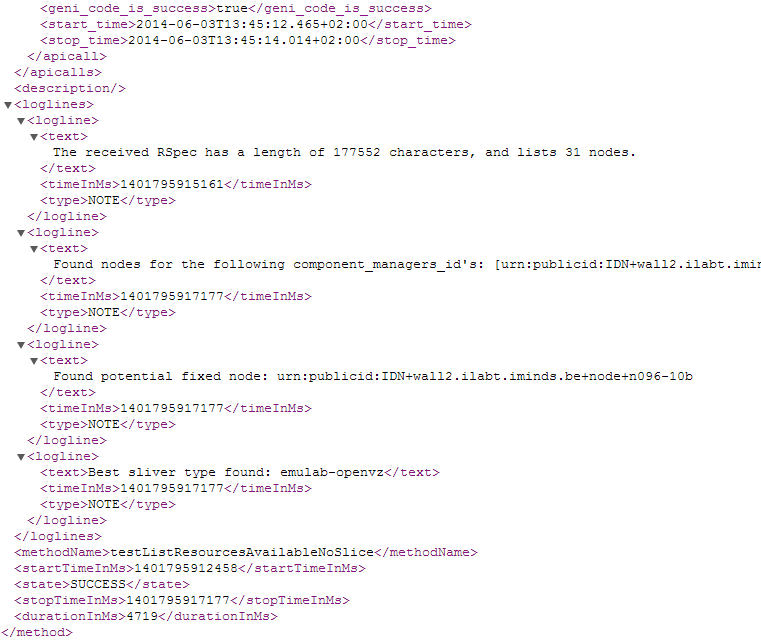
\includegraphics[width=.9\textwidth]{overviewxml}
  \caption{De originele overview in XML formaat}
\end{subfigure}
\begin{subfigure}{.45\textwidth}
  \centering
  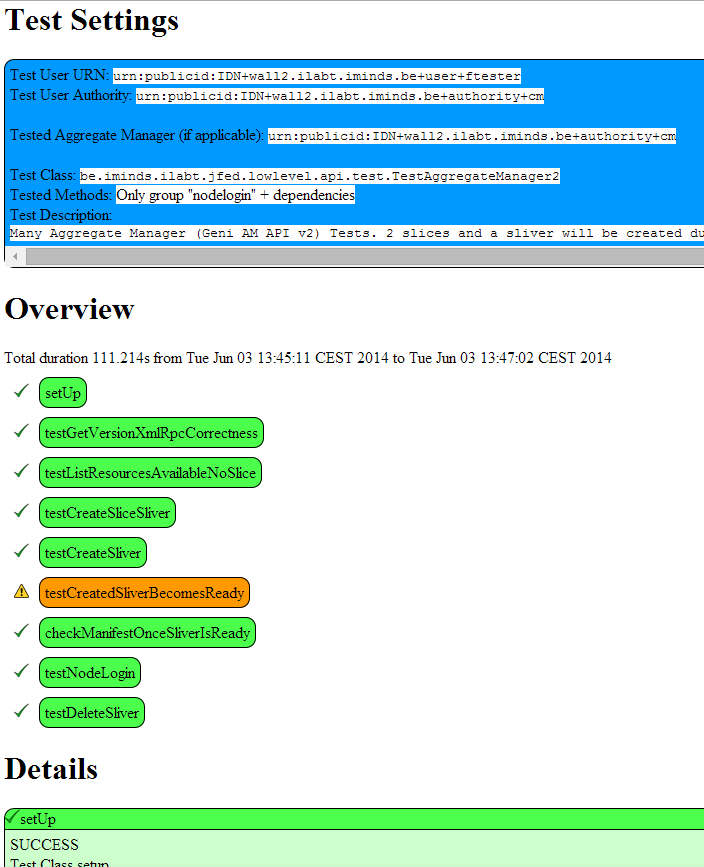
\includegraphics[width=.9\textwidth]{overviewhtml}
  \caption{Overview in html formaat}
\end{subfigure}
\caption{Naast de console uitvoer zijn ook het originele resultaat in XML formaat en het overeenkomstige HTML formaat beschikbaar.}
\end{figure}

%\documentclass[11pt]{article}
\usepackage{a4wide} 
\begin{document}
\title{Use Cases Monitoring jFed}
\author{Andreas De Lille}
\maketitle

\section{Inhoud}
In dit document wordt beschreven wat de uiteindelijke webservice moet kunnen. Daarna worden ook een aantal opmerkingen over de uitwerking gegeven. Merk op dat in deze versie enkel uitlezen van info uitgewerkt wordt. In de latere uitwerking moet het ook mogelijk zijn om de tests die uitgevoerd moeten worden te beheren via een database.
Deze database zal dan periodiek overlopen worden om de monitoring-resultaten actueel te houden.
De webservice moet de bestaande situatie opkuisen en een duidelijke interface aanbieden. Het uiteindelijke doel is dat jFed gebruik maakt van deze interface om zo een ranking van de testbeds weer te geven. Verder zal ook de huidige webinterface gebruik maken van deze interface. Indien er vragen of opmerkingen zijn bij een use case, zullen ze onder de titel opmerkingen staan.

\section{Cases}
\subsection{Ping}
De ping van de verschillende testbeds moet opgevraagd kunnen worden.
Hiervoor zou elk testbed een id moeten hebben. Het voordeel van een testbedid (en later testid) is dat men meerdere versies tegelijk kan ondersteunen. Hierdoor kan men 2 tests van het zelfde type opslaan zonder dat men problemen krijgt omdat een test van dat type al bestaat voor dat testbed. Verder moet duidelijk gemaakt worden of men enkel de laatste ping wil of het gemiddelde over een periode. Hiervoor zou een optionele parameter voorzien worden. Indien deze parameter niet ingevuld is wordt de actuele ping teruggegeven. Indien men een gemiddelde wil, moet een tijdsperiode meegeven worden. Indien de ping niet opgevraagd kan worden, wordt een foutboodschap teruggegeven.

\subsection{getVersion status}
Dit zou de Aggregate Manager server opvragen. Dit bevat o.a. het versie nummer van de aggregate manager.
Doordat er geen ssl authenticatie voor nodig is, wordt hij vaak gebruikt om de status van de server op te vragen.
Dit zou terug werken via een testbedid dat weergegeven wordt en zal enkel de actuele informatie 
terug geven. Bij een fout zal zoals altijd een foutboodschap teruggegeven worden.

\subsection{Free Resources}
Deze functie zal het aantal beschikbare resources van een testbed terug geven.
Hiervoor is een testbedid nodig.
Indien geen 2e parameter wordt weergegeven zal de actuele informatie getoond worden.
Indien een tijdsperiode meegegeven wordt zal het gemiddelde beschikbare resources over die periode teruggegeven worden. Bij een fout (als het aantal niet opgevraagd kan worden)
zal een foutboodschap teruggestuurd worden.

\subsection{Last check}
Dit zal terug geven wanneer een test voor de laatste keer is uitgevoerd op een testbed.
Hiervoor zijn dus 2 parameters nodig een testbedid en een testid.
De testid kan optioneel gemaakt worden, indien er geen testid gegeven zal het tijdstip van de laatste test op dat testbed teruggegeven worden.

\subsection{International testbed monitoring status}
Op elk testbed draait een stuk monitoring software dat periodiek zijn status aanpast in de databank.
Bij deze call moet er teruggegeven worden of status in orde is of niet, maar ook of de status periodiek aangepast wordt.

\subsection{Duration}
Dit geeft weer hoelang de laatste test op een testbed duurde.
Hiervoor is dus weer een testbedid en testid nodig.
Verder kan ook een gemiddelde opgevraagd worden, een tweede paramater door te geven die de periode voorstelt.

\subsection{Status van test}
Het moet mogelijk zijn om te zien of een test gelukt is.
Indien hij niet gelukt is moet er snel en duidelijk zichtbaar zijn bij welke stap de test is gestopt. Daarnaast moet men ook een log kunnen op vragen van de test.
Deze functie zal weer per test en testbed werken en heeft dus terug een testbedid en testid nodig.

\subsection{History van een test op een testbed}
Het moet mogelijk zijn om per testbed en per test de geschiedenis op te vragen.
Hierdoor kan men snel kijken naar de duur en de frequentie van een fout.
Zoals hierboven is ook hier weer een testid en testbedid nodig.

\subsection{History van een testbed}
Verder kan het handig zijn om per testbed een overzicht weer te geven. Dit overzicht kan data bevatten zoals wanneer was de laatste keer dat het testbed offline was en hoeveel resources zijn er gemiddeld vrij. Dit moet echter niet als functie uitwerkt worden, men kan ook meerdere calls doen om tot deze informatie te komen. Dit kan echter wel in een functie gestoken worden om het aantal calls te beperken. Zie later bij besluit.

\clearpage
\section{besluit}
\subsection{Componenten}
Ik zou werken met een database en daarboven een webservice. Deze webservice geeft dan toegang tot alle informatie. De opbouw van mijn masterproef zal bestaan in het uitschrijven van use cases gevolgd door een interface van mijn api beschikbaar te stellen. Vervolgens zal ik op basis van de service-interface een database ontwerpen. Eenmaal de database en service gekoppeld zijn kunnen loadtests uitgevoegd worden. Er zullen 2-3 grote componenten uitgewerkt worden. Een webinterface enerzijds en anderzijds integratie in jFed.
\subsubsection{Webinterface}
De huidige webinterface zal ook gebruik maken van de webservice. Het voornaamste doel van deze interface is een duidelijk overzicht tonen van de actuele situatie. Dit zou moeten zorgen dat men snel kan zien welke tests fout lopen.Indien een testfout loopt moet het snel duidelijk zijn tot welke stap hij is geraakt. Er moet dus gelinkt worden naar de logs. Deze webinterface kan verbinding maken met de webservice of rechtstreeks met de databank verbinding maken. Het voordeel hiervan is dat er minder overhead is. Een nadeel is code-duplicatie en minder eenvoudig beheer.
\subsubsection{Integratie in jFed}
Een andere component is de integratie in jFed. Het moet mogelijk zijn om bij het selecteren van een testbed weer te geven of dat testbed online is en of er nog beschikbare resources zijn.

\subsection{Opdeling}
We kunnen de use cases opdelen in 2 grote groepen, namelijk de lange en korte termijn.
\subsubsection{Lange termijn - Gemiddelde}
Enerzijds is er de gemiddelde data die moet weergeven hoe betrouwbaar een testbed is op lange termijn. De duur van die termijn kan opgegeven worden in parameters. Deze gemiddelde data zal voor een ranking zorgen van een testbed. Deze ranking heeft niet als doel om de actuele informatie weer te geven, maar om de betrouwbaarheid over lange termijn weer te geven. jFed zal deze ranking weergeven zodat een onderzoeker snel in zijn gui kan zien welk testbed betrouwbaar is.
\subsubsection{Korte termijn - Actueel}
Anderzijds is er de actuele component die de huidige toestand moet weergeven. Dit zal de overeenkomen met de laatst gemeten waarde voor die test. Deze waarde kan eventueel gecached worden om de performantie te verbeteren. De webinterface zal deze actuele informatie weergeven en voorzien in een gedetailleerd overzicht voor elke test. Dit zou het voor ontwikkelaars makkelijk moeten maken om fouten op te sporen en te verbeteren. Deze informatie kan ook in jFed ge\"{i}ntegreerd worden. Zo kan het nuttig zijn om te zien of een testbed online is en/of er resources beschikbaar zijn.

\subsection{Uitwerking}
Naast de opdeling van de use cases en de opdeling in componenten moeten we ook kijken naar performantie. Deze wordt grotendeels bepaald door de uitwerking en de gebruikte technologi\"{e}n.
\subsubsection{Calls bundelen}
Op de site https://flsmonitor.fed4fire.eu/ wordt een overzicht weergegeven van een aantal testbeds.
Met de use cases hierboven kan dit overzicht perfect worden gegenereerd. Al moet met opmerken dat elke call slechts een waarde van een test weergeeft. Er zijn dus meerdere calls nodig.
Dit kan voor overhead zorgen. Een mogelijke oplossing is calls bundelen. 
Zo kan men bv per testbedid direct een tabel met alle waarden die nodig zijn in de tabel terugsturen.
Het voordeel is de snelheidswinst, een call per testbed volstaat nu.
Het nadeel is dat dit de code minder proper maakt, 
meer functies toevoegen die dezelfde dingen doen maken de code onnodig complex.
Een oplossing is een tussenweg waarbij we een algemene get-functie maken waaraan we kunnen zeggen welke waarden we terug willen krijgen. 
Zo kunnen we bijvoorbeeld een functie get oproepen met \\
- Een array parameters={ping,version,duration \\
- Een testbedid\\
waarop de call een hashmap zal teruggeven. In die hashmap zit dan:\\
- ping  = getPing()\\
- version = getVersion()\\
- duration = getDuration()\\
Deze functie is gelijkaardig aan de history van een testbed.

\subsubsection{Technologie - php}
De tweede vraag die we ons moeten stellen is welke technologie die we gebruiken.
Aangezien de taal gekend moet zijn en op elk platform moet kunnen draaien, liggen er 2 opties voor de hand, php en java.Beide talen zijn vrij te gebruiken en draaien op zo goed als elk platform.

De tool jFed is in java geschreven.Mijn ervaring met java is ook groter dan mijn ervaring met php. Het gebruiken van java zou eventuele integratie eenvoudiger kunnen maken. Al moet men opmerken dat het hier om een webservice gaat. Een webservice zal antwoorden in een taalonafhankelijk formaat zoals json of xml. Beide talen zullen dezelfde json genereren. De keuze voor java lijkt dus al gemaakt. Toch heb ik een voorkeur op php te gebruiken. De huidige uitwerking is namelijk al volledig in php. Php is een makkelijke taal om te leren. Een ander bijkomend voordeel is dat alles wat voorzien moet worden, nu al ge\"{i}mplementeerd is.

\clearpage
\subsubsection{Type webservice - REST}
Er liggen 2 types voor de hand SOAP (Simple Object Access Protocol) en REST (Representational State Transfer). Er zijn een aantal verschillen tussen beide types. Beide zijn ondersteund door meerdere programmeertalen.Beide kunnen json/xml uitwisselen over het http protocol. Het grote verschil is dat er voor elke SOAP-service een WSDL file is. In deze file worden de functies en parameters volledig beschreven. Verder verpakt SOAP zijn berichten in een SOAP-envelop bestaande uit een SOAP-header en een SOAP-body.
REST heeft geen file waarin alles beschreven wordt. De filosofie van rest is eenvoud. Rest is volledig statusloos en veel minder strict dan SOAP. Rest heeft geen overzichtsfile waarin alles tot in details beschreven staat. Als we beide vergelijken zien we dat REST een betere performantie biedt. SOAP voorziet in meer out-of-the-box functionaliteit zoals beveiliging en transacties. Dit echter wel ten koste van performantie. Aangezien de beveiliging van monitoring informatie niet de hoogste prioriteit is, lijkt REST hier de juiste keuze te zijn. Eventuele beveiliging kan dan later toegevoegd worden.


\end{document}
%\input{keuzes}
%\input{interfacewebservice}
%\input{databank}


% De appendices:
\appendix




% De bibliografie en de index
\backmatter

\bibliography{lc-bibliografie}

\printindex                             % Om de index af te printen, niet bij een thesis.

\end{document}

